\documentclass[a4paper, 12pt, twoside]{article}
\usepackage[T2A,T1]{fontenc}
\usepackage[utf8]{inputenc}
\usepackage[english, russian]{babel}
\usepackage{graphicx}
\usepackage{ amssymb }
\usepackage[hcentering, bindingoffset = 10mm, right = 15 mm, left = 15 mm, top=20mm, bottom = 20 mm]{geometry}
\usepackage{multirow}
\usepackage{ amssymb }
\usepackage{lipsum}
\usepackage{amsmath, amstext}
\usepackage{siunitx}
\usepackage{subcaption}
\usepackage{wrapfig}
\usepackage{adjustbox}
\usepackage{enumerate, indentfirst, float}
\usepackage{capt-of, svg}
\usepackage{ctable}
\usepackage{cmap} % Улучшенный поиск русских слов в полученном pdf-файле
\newcommand*{\hm}[1]{#1\nobreak\discretionary{} 
	{\hbox{$\mathsurround=0pt #1$}}{}}

\usepackage{pscyr} % Нормальные шрифты
\usepackage[normalem]{ulem} % для подчёркиваний uline
\ULdepth = 0.16em

\usepackage{fancyhdr} %Колонтикулы
\pagestyle{fancy}
\lhead{
\includegraphics[width = 10 mm]{logo.jpg} Лабораторная работа № 3.2.6}
\rhead{\textit{\today}}

\newenvironment{bottompar}{\par\vspace*{\fill}}{\clearpage}
 
\begin{document}
\begin{titlepage}

\newcommand{\HRule}{\rule{\linewidth}{0.7mm}} % Defines a new command for the horizontal lines, change thickness here

\center % Center everything on the page
 
%----------------------------------------------------------------------------------------
%	HEADING SECTIONS
%----------------------------------------------------------------------------------------

\textsc{\LARGE Московский Физико-Технический Институт}\\[1,5cm] % Name of your university/college
\textsc{\Large Кафедра общей физики}\\[0.5cm] % Major heading such as course name
\textsc{\large Лабораторная работа \textnumero  3.3.4}\\[0.5cm] % Minor heading such as course title

%----------------------------------------------------------------------------------------
%	TITLE SECTION
%----------------------------------------------------------------------------------------

\HRule
\\[0.4cm]
{ \huge \bfseries Эффект Холла в полупроводниках.}
\\[0.2cm] % Title of your document
\HRule
\\[1.5cm]


 
%----------------------------------------------------------------------------------------
%	AUTHOR SECTION
%----------------------------------------------------------------------------------------

\begin{minipage}{0.4\textwidth}
	\begin{flushleft} \large
		\textbf{Автор:}\\
		Глеб Уваркин \\
		615 группа
	\end{flushleft}
\end{minipage}
~
\begin{minipage}{0.4\textwidth}
	\begin{flushright} \large
		\textbf {Преподаватель:} \\
		Андрей Александрович Заболотных % Supervisor's Name
	\end{flushright}
\end{minipage}

\begin{bottompar}
	\begin{center}
		
\includegraphics[width = 80 mm]{logo.jpg}
	\end{center}
	{\large \today}

\end{bottompar}
\vfill % Fill the rest of the page with whitespace

\end{titlepage}

{\Large \uline { \textbf  {Цель работы:}}}

\vspace{2mm}
Измерение подвижности и концентрации носителей заряда в полупроводниках.
\vspace{\baselineskip}

{\Large \uline { \textbf  {В работе используются:}}}

\vspace{2mm}

Электромагнит с источником питания GPR, батарейка 1,5 В, амперметр, реостат, цифровой вольтметр В7-78/1, милливеберметр, образцы легированного германия.

\section{Теоретическая часть}

\subsection{Дырки}

Эффект Холла, возникающий в проводниках, происходит из-за наличия некоторого количества свободных электронов в зоне проводимости и такого же количества дырок в валентной зоне. Чтобы понять причину образования дырок, нужно рассмотреть дырочную проводимость.


Дырочную проводимость можно объяснить при помощи следующей аналогии: если представить ряд людей, сидящих в аудитории, где нет запасных стульев. Когда кто-нибудь из середины ряда хочет уйти, он      перелезает через спинку стула в пустой ряд и уходит. Здесь пустой ряд — аналог зоны проводимости, а ушедшего человека можно сравнить со свободным электроном.
Теперь представим, что ещё кто-то пришёл и хочет сесть. Из пустого ряда плохо видно, поэтому там он не садится. Вместо этого человек, сидящий возле свободного стула, пересаживается на него, вслед за ним это повторяют и все его соседи. Таким образом, пустое место как бы двигается к краю ряда. Когда это место окажется рядом с новым зрителем, он сможет сесть.
В этом процессе каждый сидящий передвинулся вдоль ряда. Если бы зрители обладали отрицательным зарядом, такое движение было бы  \textit{электрической проводимостью}. Если вдобавок стулья заряжены положительно, то ненулевым суммарным зарядом будет обладать только свободное место. Это простая модель, показывающая как работает \textit{дырочная проводимость}. Однако на самом деле, из-за свойств кристаллической решётки, дырка не локализована в определённом месте, как описано выше, а размазана по области размером во много сотен элементарных ячеек.

\subsection{Эффект Холла}


\begin {figure}[H]
\begin{center}
	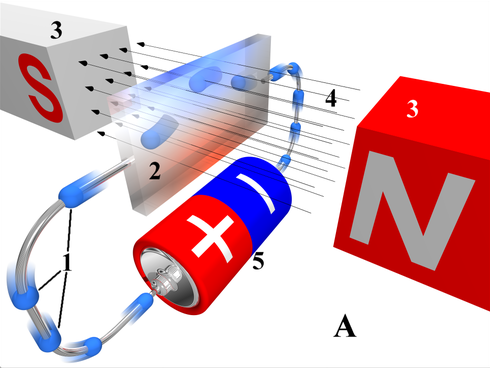
\includegraphics[width = 0.4 \textwidth]{Hall_effect}
	\caption{Пример действия эффекта Холла на свободные заряды}
\end{center}
\end {figure}


Магнитного поле в проводнике действует на свободные электроны в зоне проводимости, поэтому между гранями наблюдается добавочная разность потенциалов, связанная с силой Лоренца. 

$$\boldsymbol{F_\text{Л}}  = -e \boldsymbol{E} - e \langle \boldsymbol{\upsilon} \rangle \times \boldsymbol{B},$$
где $e$ - абсолютная величина заряда электрона, $\boldsymbol{B}$ - индукция магнитного поля, $\boldsymbol{E}$ - напряженность электрического поля, $ \langle \upsilon \rangle$ - средняя скорость заряда.

Из этого выражения получим разность потенциалов между двумя гранями:

\begin{equation}
U = -E_zl = - | \langle \upsilon \rangle | B l
\label{eq:pot_dif}
\end{equation}

С этой возникшей разностью потенциалов и связан Эффект Холла.

Далее, если выразить ток:
$$ I = ne |\langle \upsilon \rangle |  l a$$
И совместить его с \ref{eq:pot_dif}, получим ЭДС Холла:

\begin{equation}
\mathcal{E}_x = U = - \dfrac{IB}{nea} = -R_x \cdot \dfrac{IB}{a},
\label{eq: Hall}
\end{equation}

где $R_x = \dfrac{1}{ne}$ называется \textit{постоянной Холла.}

\newpage

\section{Установка и параметры измерения}
\begin{minipage}{0.6 \linewidth}
	\begin{figure}[H]
	\centering
	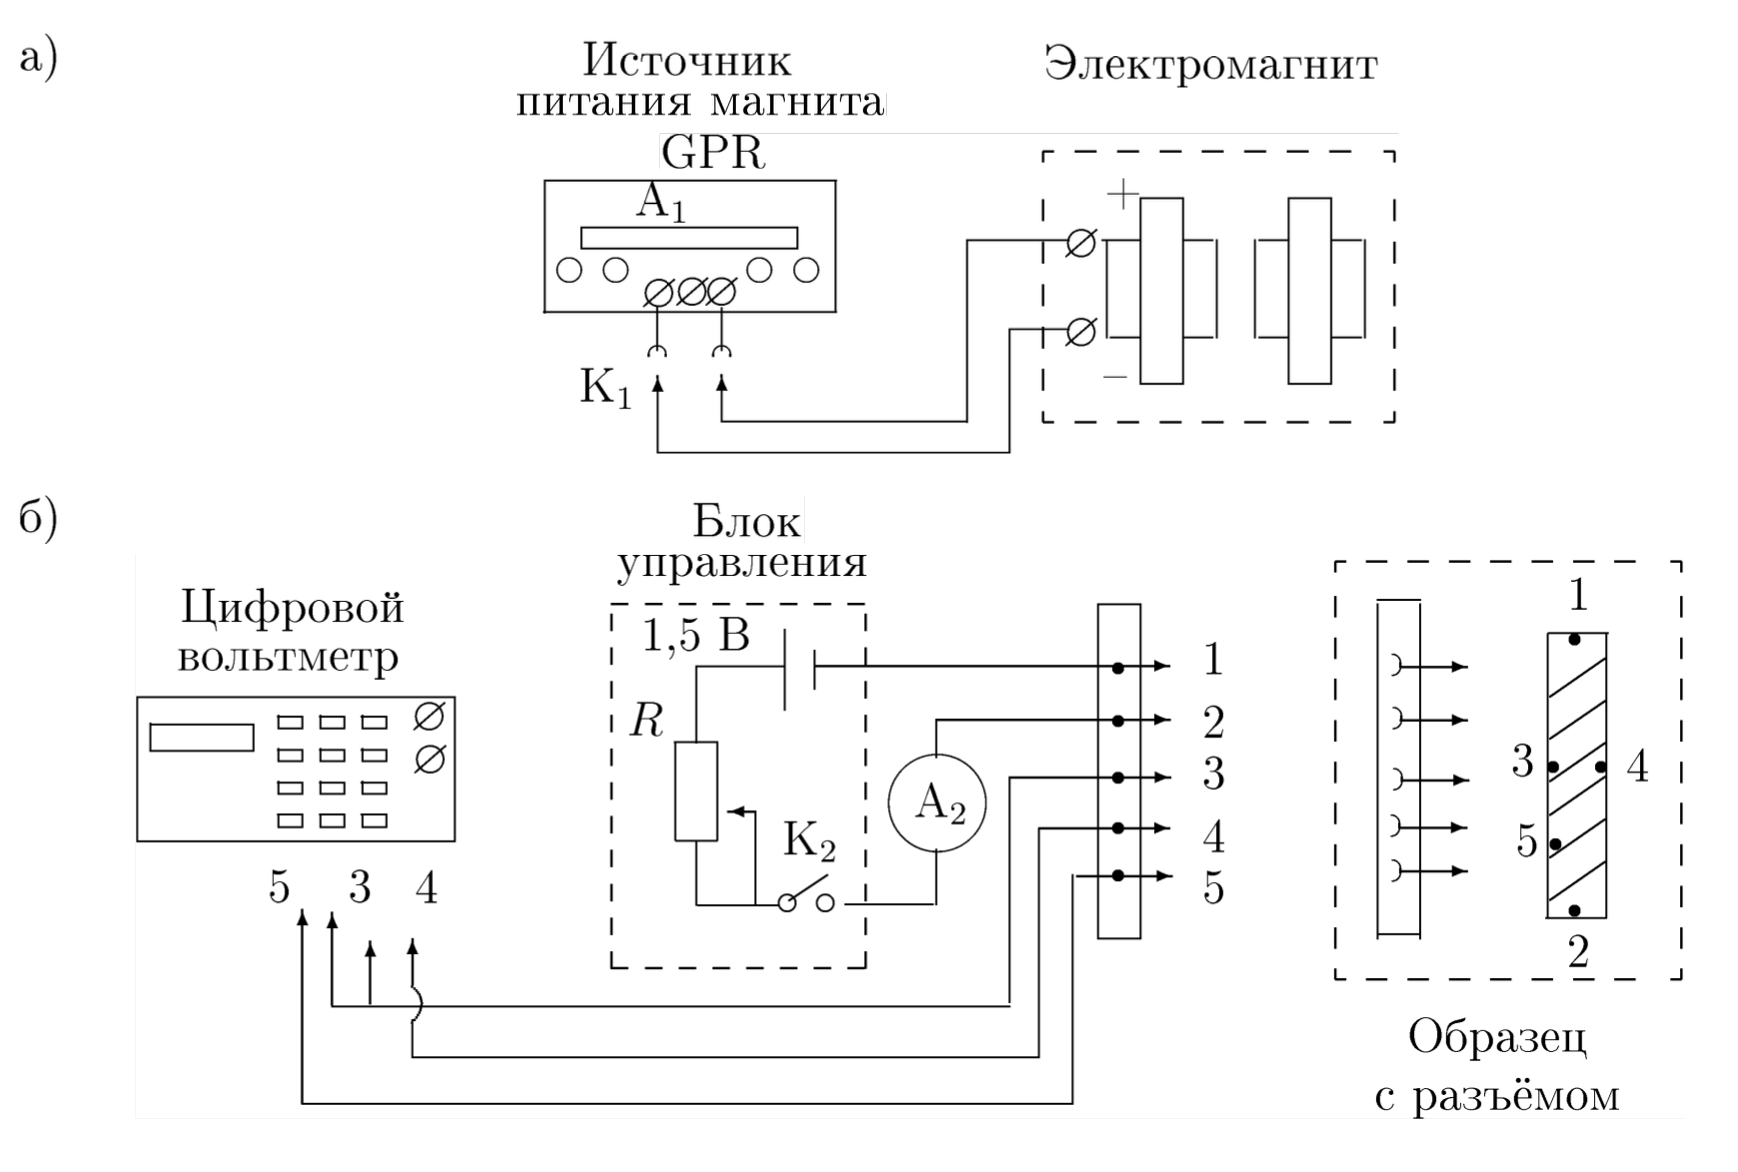
\includegraphics[width = \textwidth]{Scheme1}
	\caption{Схема установки для измерения эффекта Холла в полупроводниках}
	\end{figure}
\end{minipage}
~
\begin{minipage}{0.3\linewidth}
	$$\text{Параметры установки:}$$
	$$a = 2.2 \text{ мм}$$
	$$L_{35} = 6 \text{ мм}$$
	$$l = 7 \text{ мм}$$
\end{minipage}
 
 ~

В нашей установке вдоль длинной стороны образца будет течь ток, величина которого регулируется реостатом $R_2$. Так как он помещен в электромагнит, между точками \textit{3 и 4} будет возникать разность потенциалов $U_{34}$, которую мы будем измерять. 

Однако между точками \textit{3 и 4} будет возникать некоторое дополнительное падение напряжения $U_{0}$, так как эти точки оказываются не на одной эквипотенциали. Исключить это влияние можно с помощью изменения направления магнитного поля: в одном случае $U_{34} = U_{0} - \mathcal{E}_x $, в другом  $U_{34} = U_0 - \mathcal{E}_x $. Тогда с помощью полуразности избавимся от $U_{0}$ в наших измерениях. 

\begin{figure}[H]
	\begin{center}
		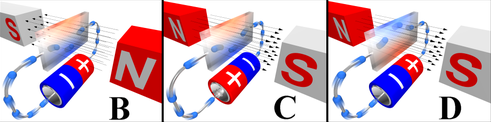
\includegraphics[width = 0.6 \textwidth]{Hall_dif}
		\caption{Эффект Холла при различных направлениях магнитного поля и тока через образец}
	\end{center}
\end{figure}

\newpage

\section{Обработка результатов.}
\subsection{Градуировка электромагнита.}
С помощью милливеберметра исследуем зависимость индукции $B$ магнитного поля в зазоре электромагнита от тока через обмотки магнита. Запишем результат в таблицу (\ref{t1}).

\begin{table}[H]
	\centering
	\caption{Зависимость $B = f(I_{M})$.}
	\label{t1}
	\begin{tabular}{c|cccccccc} \toprule
		$J_{M},~\text{А}$ & 0    & 0.3  & 0.6  & 0.9  & 1.2  & 1.5  & 1.8   & 2.1   \\
		$B,~\text{мТл}$   & 0.28 & 2.22 & 4.58 & 6.67 & 8.61 & 9.86 & 10.83 & 11.53 \\ \bottomrule
	\end{tabular}
\end{table}

Построим график этой зависимости:

	\begin{figure}[H]
	\centering
	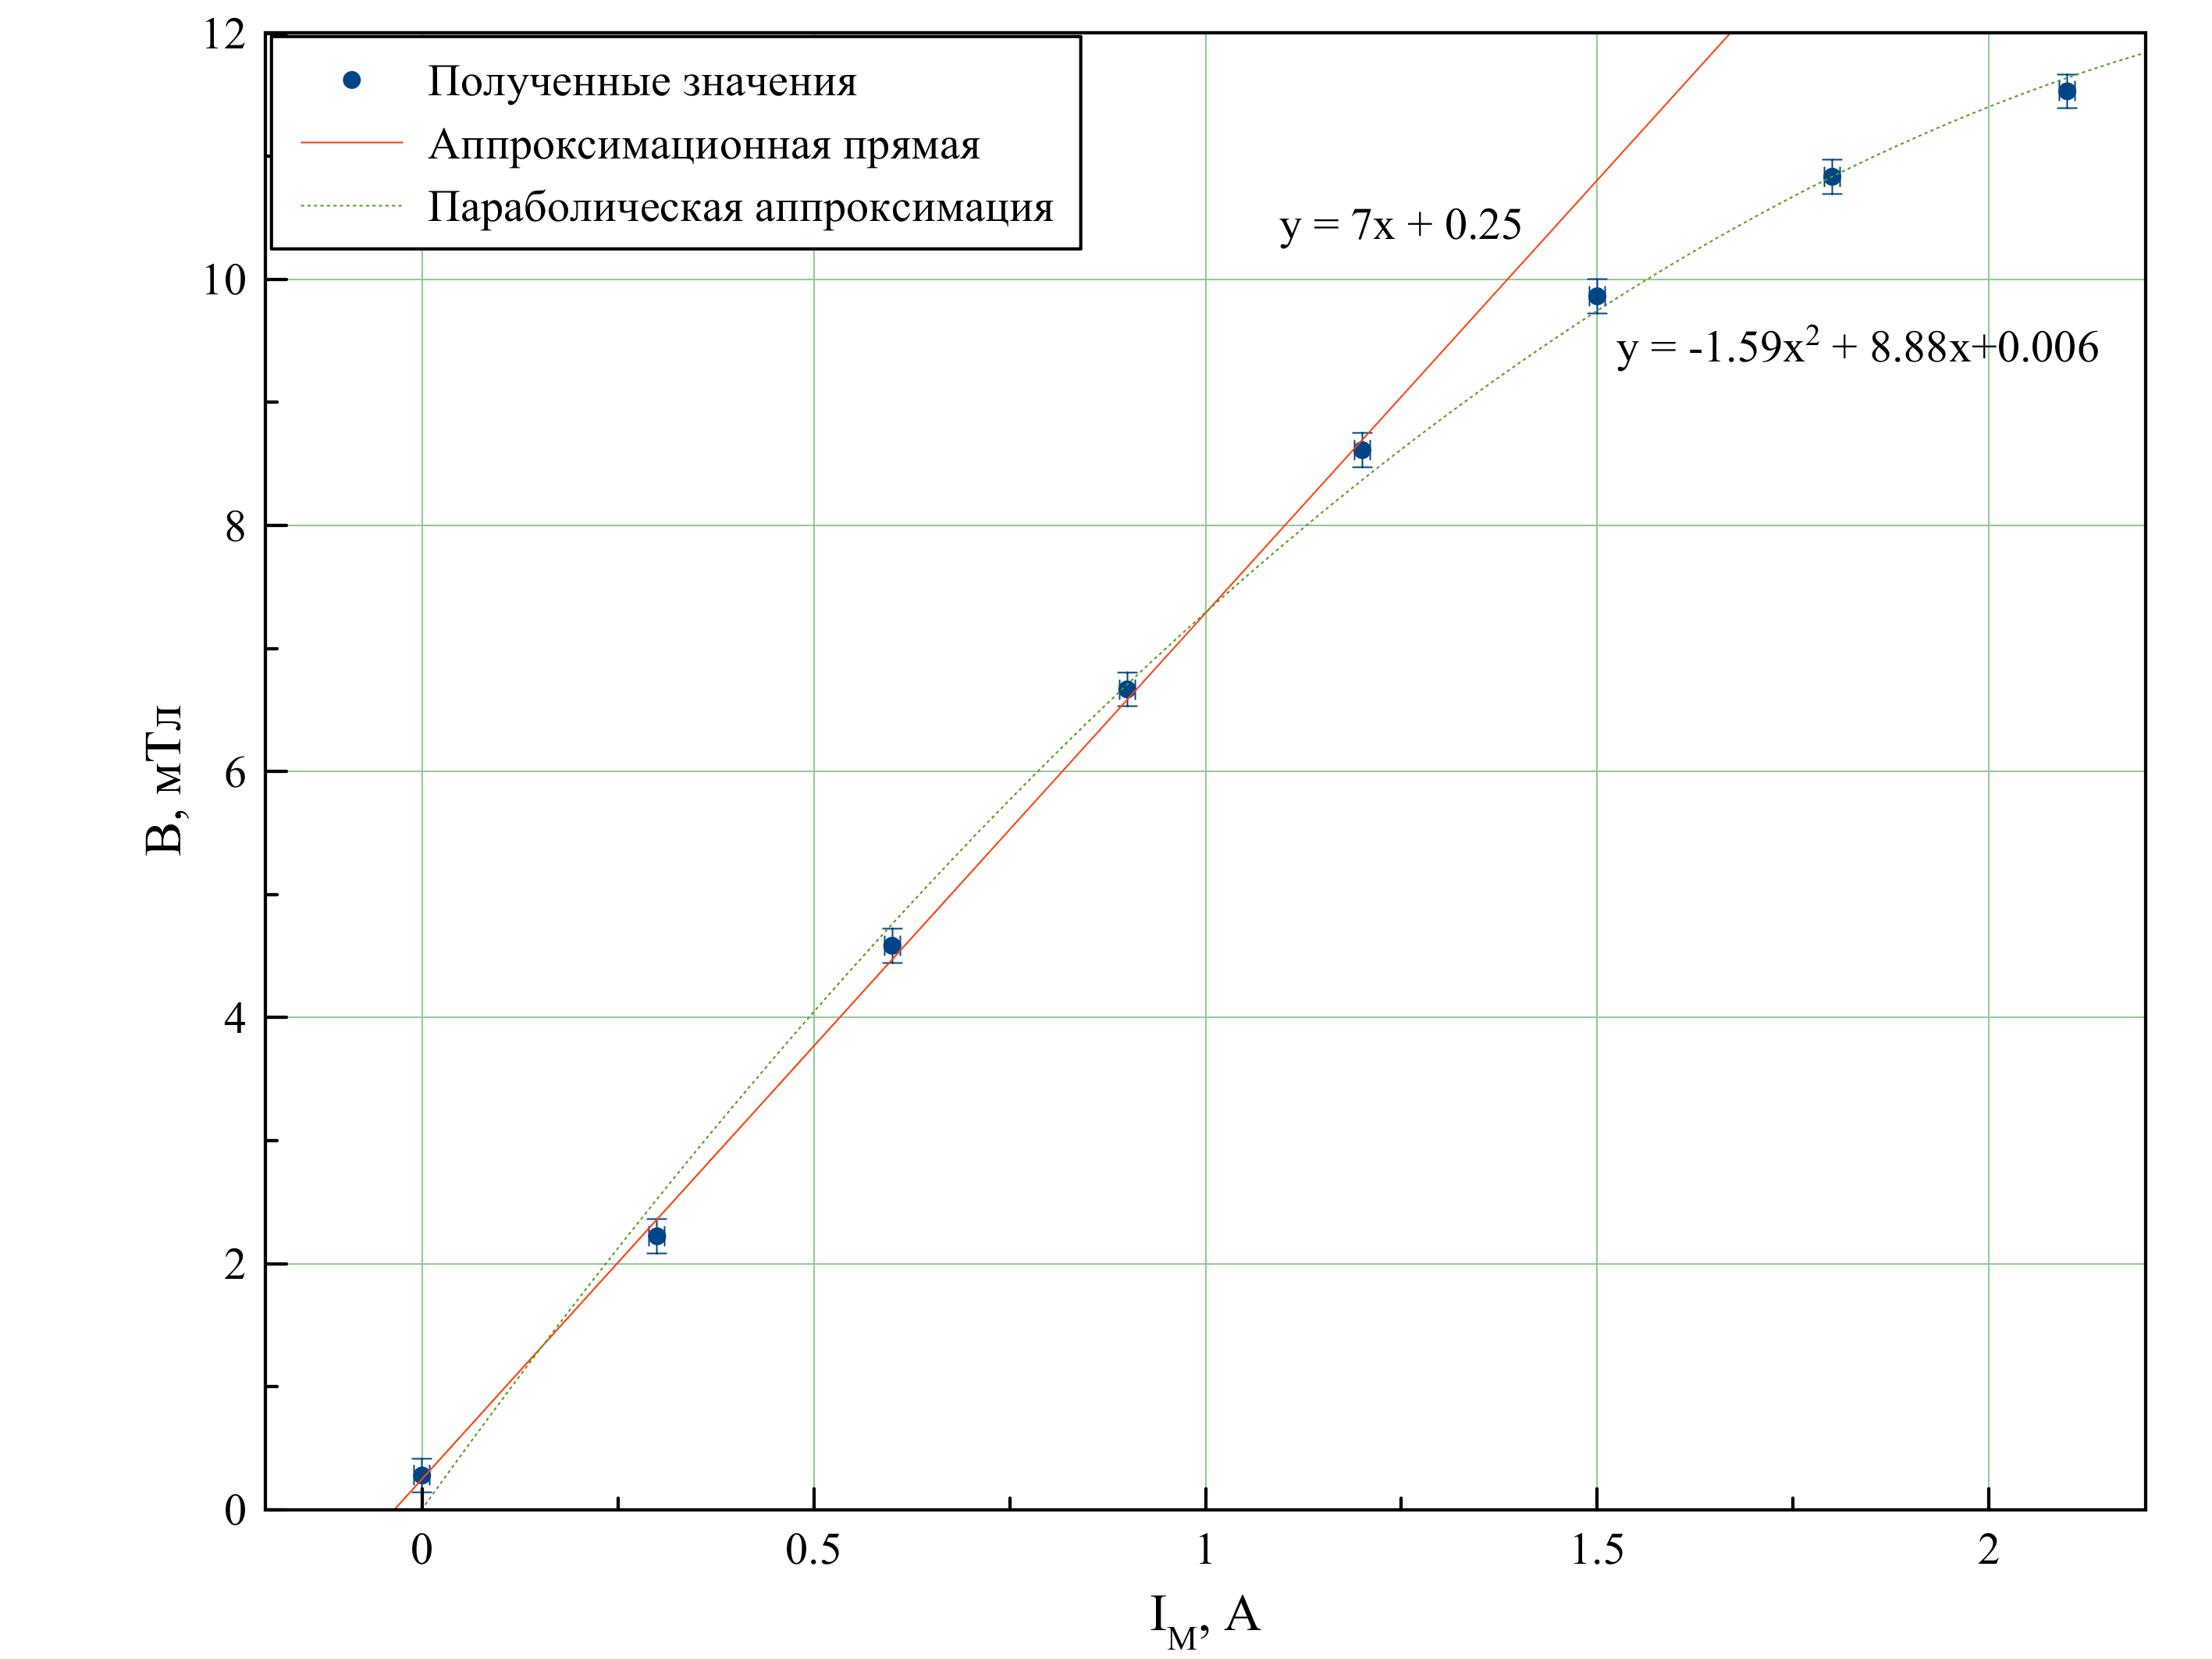
\includegraphics[width = 0.8 \textwidth]{grph1}
	\caption{График зависимости $B = f(I_M)$.}
	
\end{figure}

\subsection{Измерение ЭДС Холла.}
Снимем зависимость ЭДС Холла от величины магнитной индукции $B$ при разных значениях тока $I$ через образец. Построим на одном листе семейство характеристик $\mathcal{E}_x \hm{=} f(B).$
\begin{table}[H]
	\centering
	\label{my-label}
	\caption{Зависимость ЭДС Холла от магнитного поля}
	\begin{tabular}{c|c|c|c|c|c|c|c|c|c|c}
		\toprule
		\multirow{2}{*}{$I, \text{ мА}$} & \multirow{2}{*}{$U_0, \text{ мВ}$} & $I_M, \text{ А}$                                                      & 0    & 0.3    & 0.6    & 0.9    & 1.2    & 1.5   & 1.8    & 2.1    \\% \cline{3-11}
		&                                    & $B, \text{ мТл}$                                                        & 27.8  & 222.2  & 458.3  & 666.7  & 861.1  & 986.1  & 1083.3  & 1152.8  \\ \midrule
		\multirow{2}{*}{0.3}             & \multirow{2}{*}{0.066}              & $U, \text{мВ}$                                                         & 0.066  & 0.095 & -0.122 & 0.145 & 0.164 & 0.178 & 0.185 & 0.192 \\% \cline{3-11} 
		&                                    & $\mathcal{E}_x,$  $ \text{мВ}$ & 0 & 0.029 & 0.056 & 0.079 & 0.098 & 0.112 & 0.119 & 0.126 \\ \midrule	
		\multirow{2}{*}{0.4}             & \multirow{2}{*}{0.087}             & $U, \text{мВ}$                                                         & 0.090  & 0.126 & 0.162 & 0.194 & 0.218 & 0.236 & 0.247 & 0.255 \\% \cline{3-11} 
		&                                    & $\mathcal{E}_x,$   $\text{мВ}$& 0.003 & 0.039 & 0.075 & 0.107 & 0.131 & 0.149 & 0.160 & 0.168 \\ \midrule
		\multirow{2}{*}{0.5}             & \multirow{2}{*}{0.108}             & $U, \text{мВ}$                                                         & 0.113  & 0.159 & 0.202 & 0.243  & 0.274 & 0.295 & 0.308 & 0.318 \\% \cline{3-11} 
		&                                    & $\mathcal{E}_x,$   $\text{мВ}$ & 0.005 & 0.051 & 0.094 & 0.135  & 0.166 & 0.187 & 0.200 & 0.210 \\ \midrule
		\multirow{2}{*}{0.6}             & \multirow{2}{*}{0.130}             & $U, \text{мВ}$                                                         & 0.135  & 0.188 & 0.245 & 0.289 & 0.328 & 0.355 & 0.371 & - \\% \cline{3-11} 
		&                                    & $\mathcal{E}_x,$ $ \text{мВ}$& 0.005 & 0.058 & 0.115 & 0.159 & 0.198 & 0.225 & 0.241 & - \\ \midrule
		\multirow{2}{*}{0.7}             & \multirow{2}{*}{0.153}             & $U, \text{мВ}$                                                        & 0.159  & 0.221 & 0.285 & 0.340 & 0.385 & 0.415 & 0.434 & - \\% \cline{3-11} 
		&                                    & $\mathcal{E}_x,$   $\text{мВ}$ & 0.006 & 0.068 & 0.132 & 0.187 & 0.232 & 0.262 & 0.281 & - \\ \midrule
		\multirow{2}{*}{0.8}             & \multirow{2}{*}{0.174}             & $U, \text{мВ}$                                                         & 0.180  & 0.253 & 0.325 & 0.395 & 0.443 & 0.473 & 0.494 & - \\% \cline{3-11} 
		&                                    & $\mathcal{E}_x,$  $ \text{мВ}$ & 0.006 & 0.079 & 0.151 & 0.221 & 0.269 & 0.299 & 0.320 & - \\ \midrule
		\multirow{2}{*}{0.9}             & \multirow{2}{*}{0.196}             & $U, \text{мВ}$                                                          & 0.204  & 0.288 & 0.365 & 0.435 & 0.494 & 0.532 & 0.556 & - \\% \cline{3-11} 
		&                                    & $\mathcal{E}_x,$  $\text{мВ}$& 0.008 & 0.092 & 0.189 & 0.239 & 0.298 & 0.336 & 0.360 & - \\ \midrule
		\multirow{2}{*}{1.0}               & \multirow{2}{*}{0.218}             & $U, \text{мВ}$                                                        & 0.227  & 0.318 & 0.408 & 0.485 & 0.549 & 0.592 & 0.619 & - \\% \cline{3-11} 
		&                                    & $\mathcal{E}_x,$  $\text{мВ}$ & 0.009 & 0.100 & 0.190 & 0.267 & 0.331 & 0.374 & 0.401 & - \\ \midrule
		\multirow{2}{*}{1.0}               & \multirow{2}{*}{0.220}              & $U, \text{мВ}$                                                         & 0.212  & 0.119  & 0.039  & -0.033  & -0.088  & -0.127  & -0.150  & -  \\% \cline{3-11} 
		&                                    & $\mathcal{E}_x,$ $ \text{мВ}$ & -0.008  & -0.101  & -0.181  & -0.253  & -0.308  & -0.347  & -0.370  & -  \\ \bottomrule[0.65mm]
	\end{tabular}
\end{table}


\begin{figure}[H]
	\begin{center}
		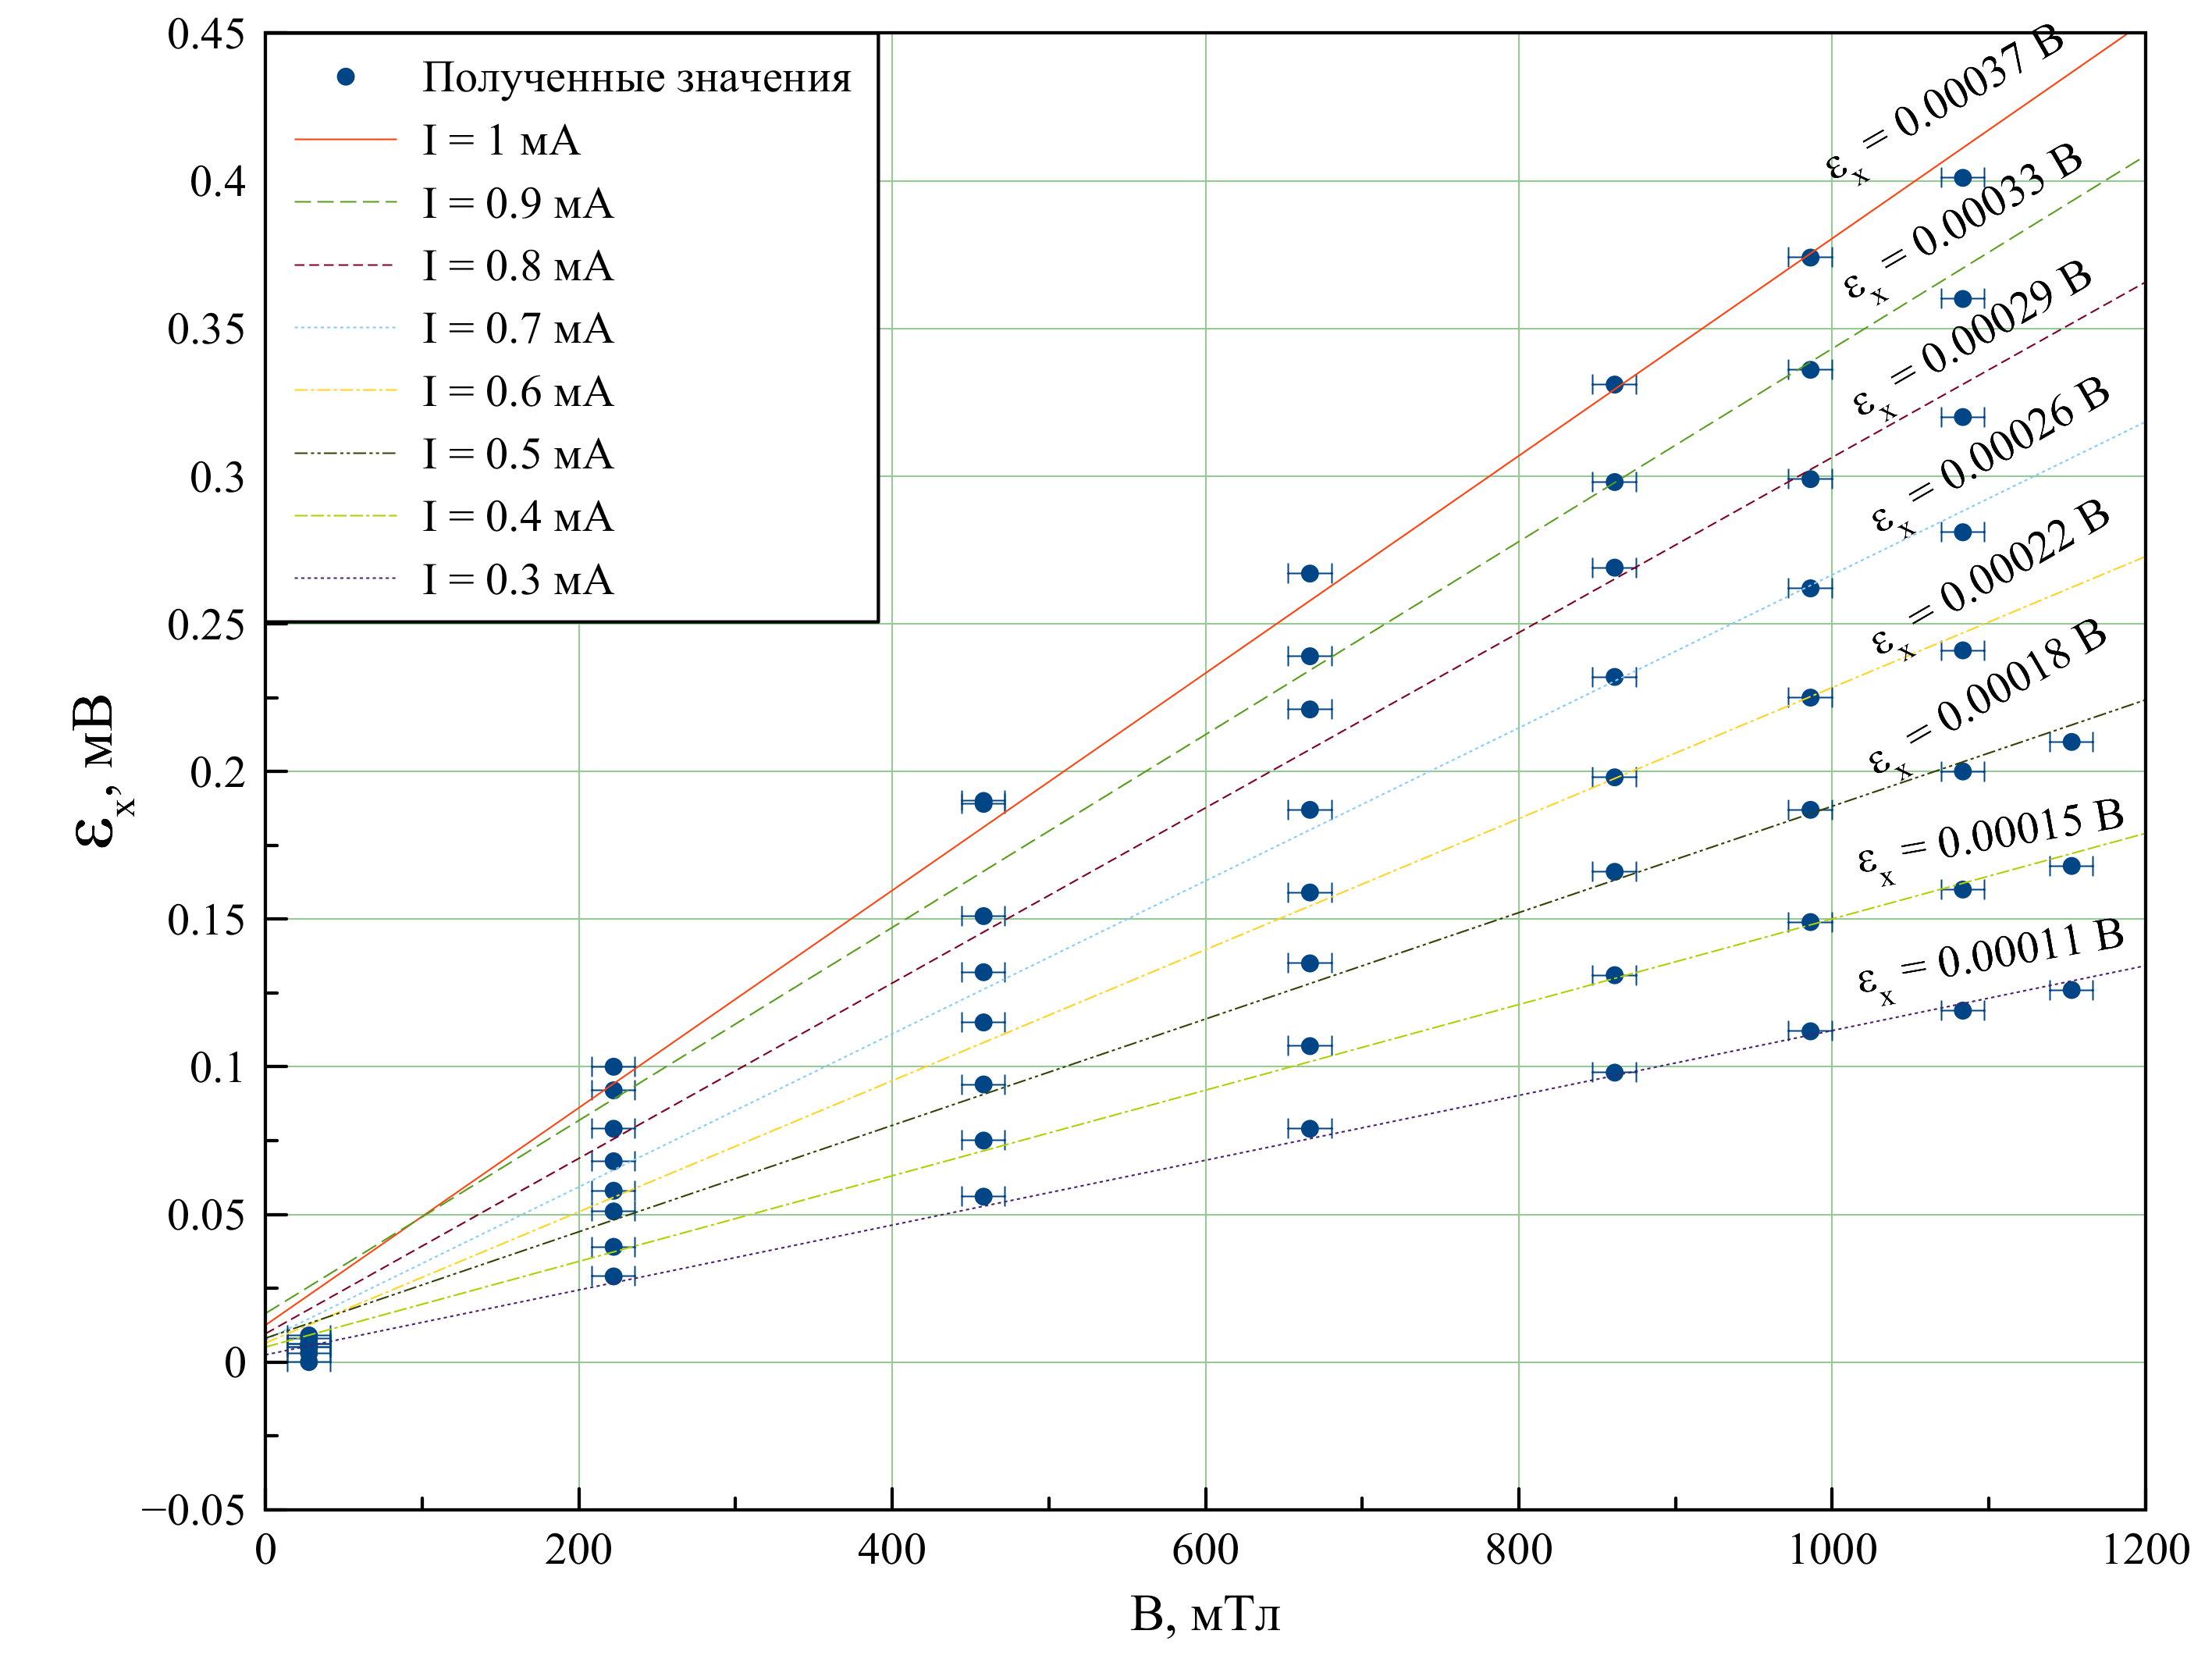
\includegraphics[width = 0.8 \textwidth]{grph2}
		\caption{График зависимости $\mathcal{E}_x = f(B)$ при разных значениях тока $I$ через образец.}
	\end{center}
\end{figure}

С помощью метода МНК определим угловые коэффициенты $K(I) = \Delta \mathcal{E} / \Delta B$ полученных прямых. Построим график $K = f(I)$.

\begin{table}[H]
	\centering
	\caption{Зависимость углового коэффициента от силы тока.}
	\begin{tabular}{c|cccccccc} \toprule
		$I,~\text{мА}$          & 0.3    & 0.4    & 0.5    & 0.6    & 0.7    & 0.8    & 0.9    & 1      \\
		$K,~\text{мВ/Тл}$        & 0.11  & 0.15  & 0.18  & 0.22  & 0.26  & 0.29  & 0.33  & 0.37  \\ \midrule
		$\sigma_K,~\text{мВ/Тл}$ & 0.003 & 0.003 & 0.004 & 0.005 & 0.005 & 0.009 & 0.012 & 0.009 \\
		$\sigma_I,~\text{мА}$   &  \multicolumn{8}{c}{0.01}   \\ \bottomrule                                          
	\end{tabular}
\end{table}

\begin{figure}[H]
	\begin{center}
		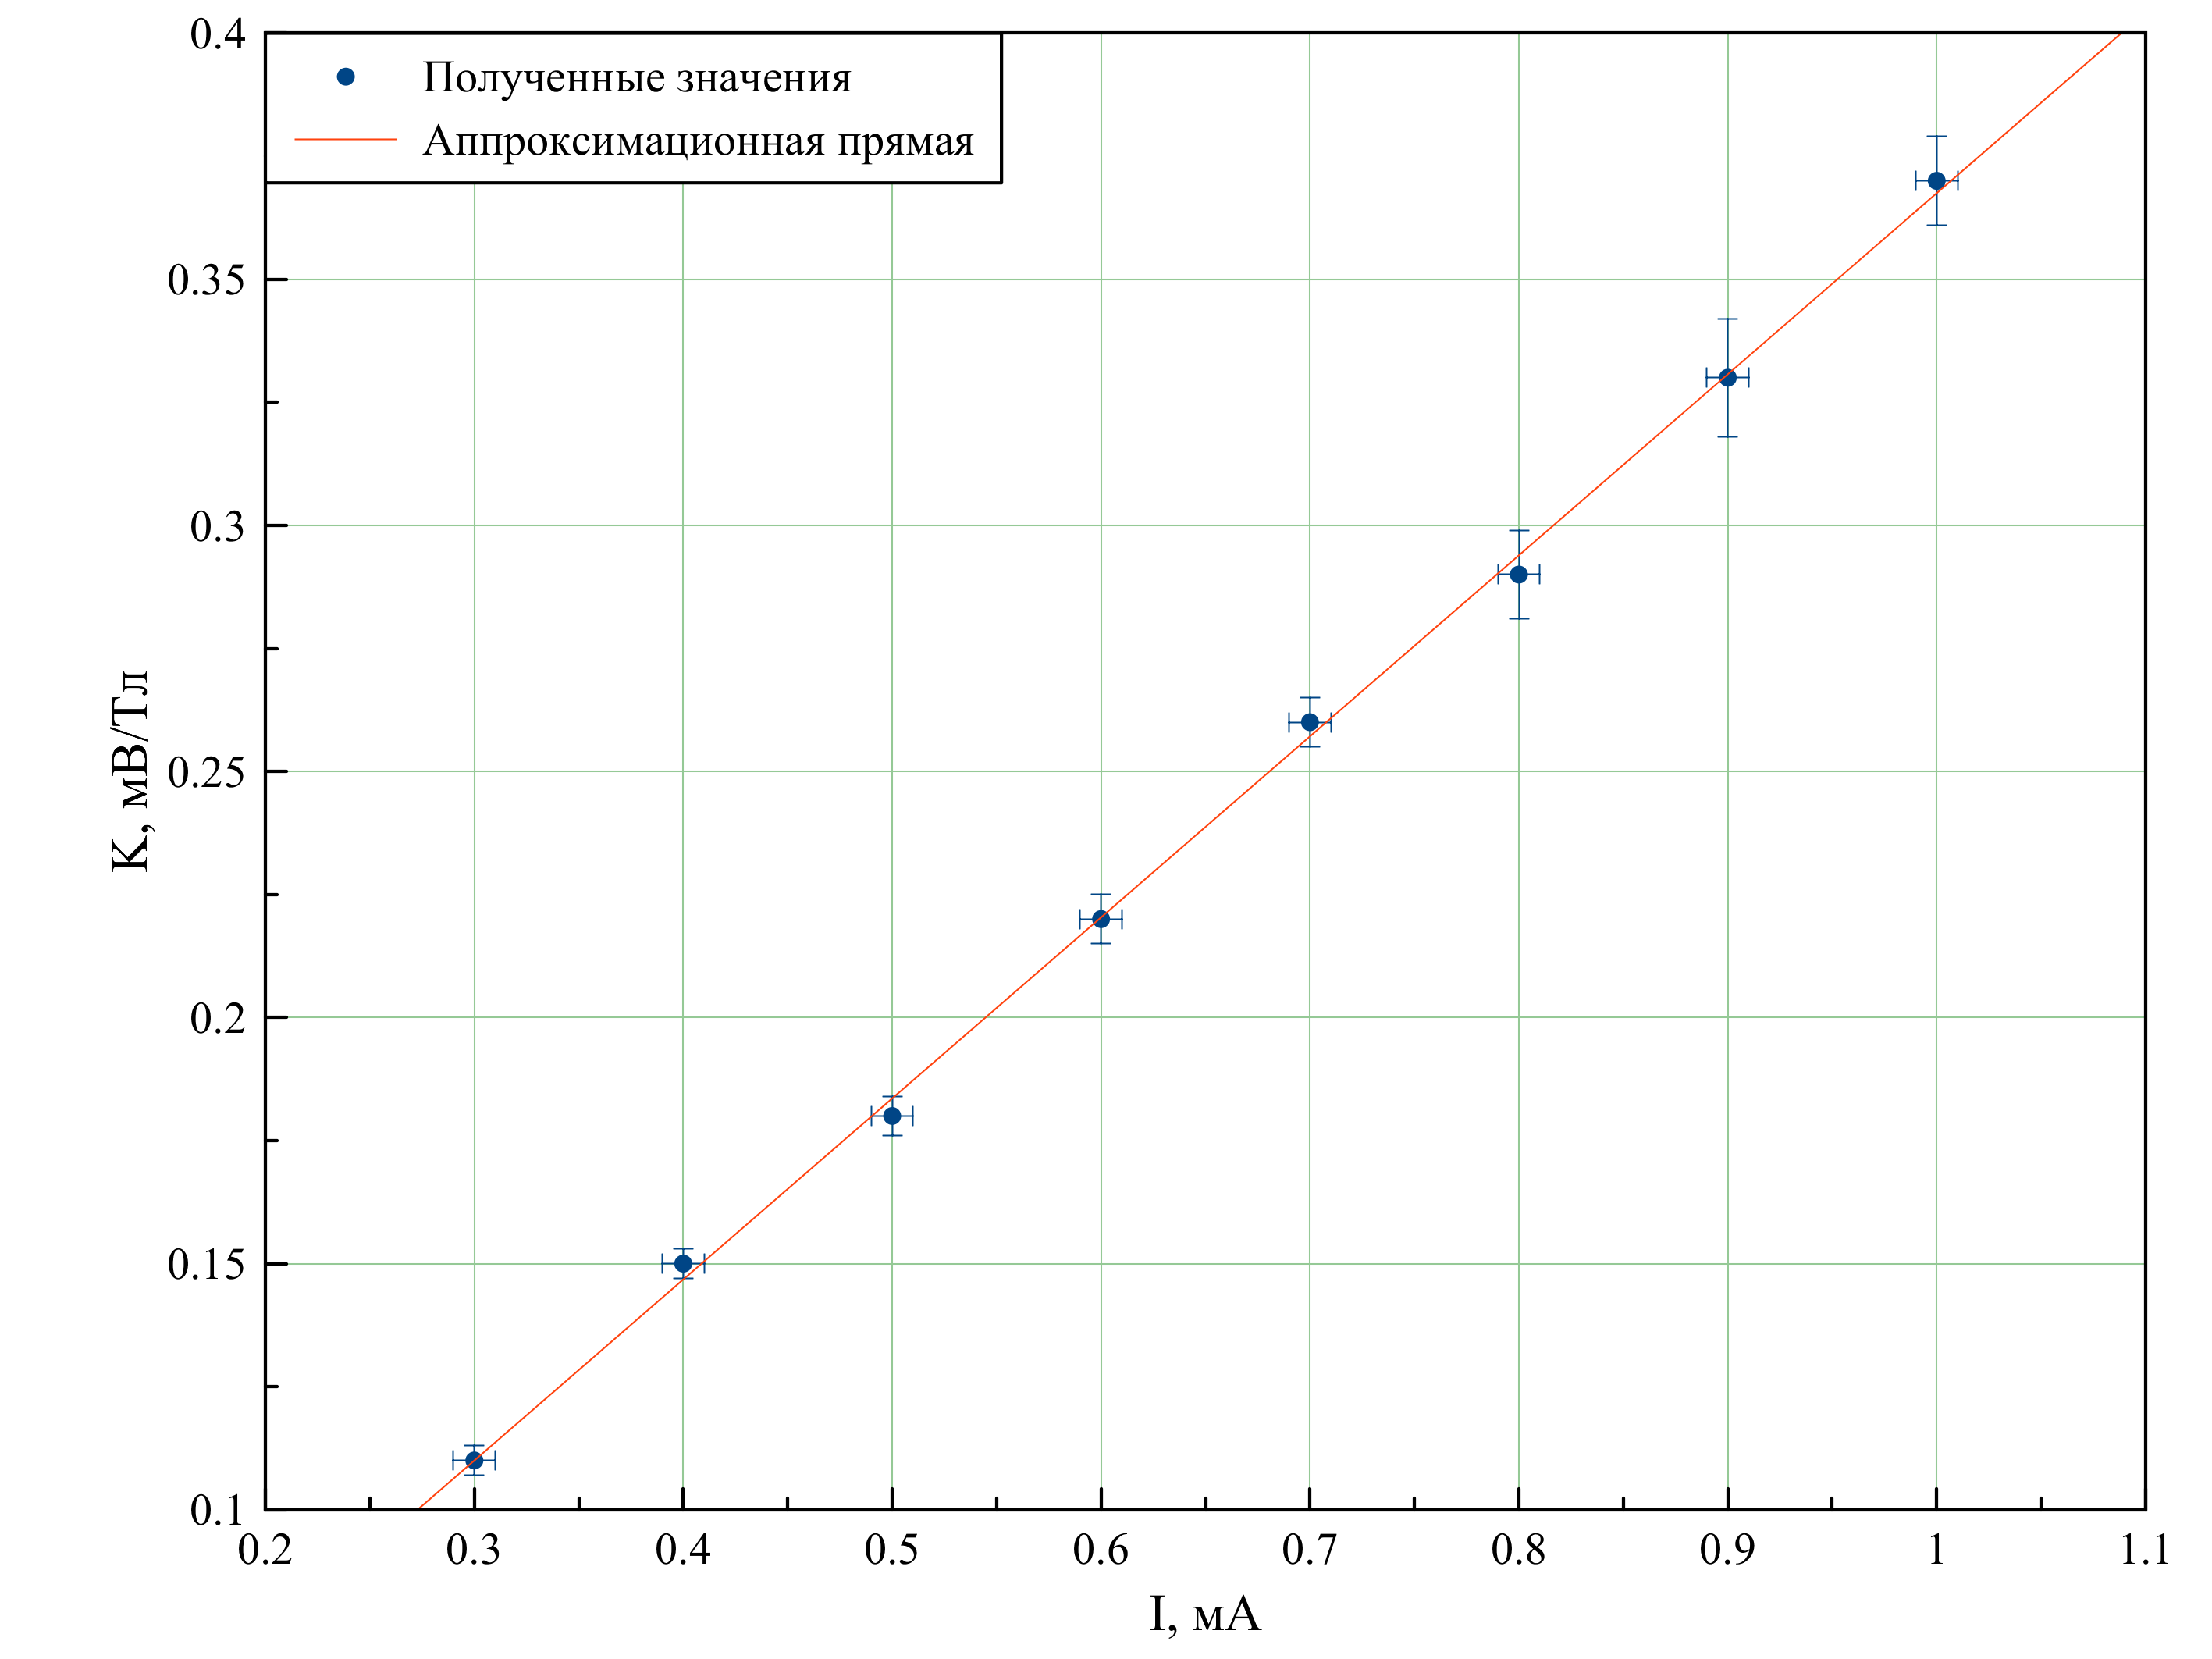
\includegraphics[width = 0.8 \textwidth]{grph3}
		\caption{График $K = f(I)$.}
	\end{center}
\end{figure}

Рассчитаем угловой коэффициент прямой с помощью МНК:
$$k = \dfrac{<K\cdot I> - <K><I>}{<I^2> - <I>^2} \simeq 0.368~ \frac{\text{В}}{\text{Тл}\cdot \text{А}}$$

$$\sigma_k = \dfrac{1}{\sqrt{8}}\sqrt{\dfrac{<K^2>-<K>^2}{<I^2>-<I>^2}-k^2} \simeq 0.004~\frac{\text{В}}{\text{Тл}\cdot \text{А}}$$

Из формулы \eqref{eq: Hall} посчитаем постоянную Холла:
$$R_x = -\dfrac{\mathcal{E}_x}{IB}\cdot a = -k\cdot a =  -(8.1 \pm 0.1) \cdot 10^{-4}~\text{м}^3/\text{Кл}.$$

Рассчитаем концентрацию $n$ носителей тока в образце:
$$n = \dfrac{1}{R_x e} \simeq (7.7 \pm 0.1) \cdot 10^{21}~1/\text{м}^3$$

Рассчитаем удельную проводимость $\sigma$ германия с помощью $U_{35} = 2.56~\text{мВ}$:
$$\sigma = \dfrac{IL_{35}}{U_{35}al} \simeq 152 \pm 3~(\text{Ом$\cdot$м})^{-1} $$

Вычислим подвижность $b$ носителей тока:
$$b = \dfrac{\sigma}{en} \simeq (1232 \pm 27)~\frac{\text{см}^2}{\text{В$\cdot$с}}~()$$


Запишем результаты расчётов в таблицу:
\begin{table}[H]
	\centering
	\caption{Итоговые значения.}
	\label{titog}
	\begin{tabular}{c|c|c|c|c|} \toprule
		\begin{tabular}[c]{@{}c@{}}$R_x \pm \Delta R_x,$\\ $10^{-4}~\text{м}^3/ \text{Кл}$\end{tabular} & Знак носителя & \begin{tabular}[c]{@{}c@{}}$n\pm \Delta n,$\\ $10^{21}~ (\text{м}^3)^{-1}$\end{tabular} & \begin{tabular}[c]{@{}c@{}}$\sigma \pm \Delta \sigma ,$\\ $(\text{Ом$\cdot$м})^{-1}$\end{tabular} & \begin{tabular}[c]{@{}c@{}}$b\pm \Delta b,$\\ $10^4~ \text{см}^2/(\text{В$\cdot$с})$\end{tabular} \\ \midrule
		$-8.1\pm0.1$                                                                                      & -             & $7.7\pm 0.1$                                                                             & $152\pm 3$                                                                                          & $1232\pm 27$      \\ \bottomrule                                                                               
	\end{tabular}
\end{table}

\section{Вывод.}

В данной лабораторной работе был изучен эффект Холла, определены подвижность и концентрация носителей тока, а также их знак в легированном германии.



\end{document}

